\documentclass[a4paper]{exam}
\usepackage[margin=1in]{geometry}
\usepackage{amsmath, amsfonts}
\usepackage{pythonhighlight}
\usepackage{graphicx} %package to manage images
\graphicspath{ {./images/} }

\printanswers
\begin{document}
\begin{center}
{\Large \textbf{Spring 2024}}\vspace{1.0em}\\
{\Large \textbf{CS 412 (Algorithms: Design and Analysis)}}\vspace{1.0em}\\
{\Large \textbf{Weekly Challenge 02: Sorting}}\vspace{1.0em}\\
{\Large Announced: Friday, January 19, 2024.}\\
\vspace{.25em}
{\Large Deadline: Friday, January 26 , 2024 (11:59 pm PKT).}\\ 
\vspace{.3em}
{\Large Total marks: 1.}
\vspace{.5em}\\
\end{center}
Instructions: Submit \textbf{individually} your solution as a PDF with the file name as your $studentID.pdf$; typeset in LaTeX. You must submit your solution on Canvas.

\centerline{\rule{.7\textwidth}{1pt}}

\begin{questions}
\question[1]
A decision tree is a binary tree that represents the comparisons between elements that are performed by a particular sorting algorithm operating on an input of a given size. Control, data movement, and all other aspects of the algorithm are ignored. The leaf nodes represent all possible permutations (arrangements) of the input array. For example, the following is a decision tree of the bubble sort algorithm for $n=3$, where $n$ is the total number of elements in an array.
\begin{center}
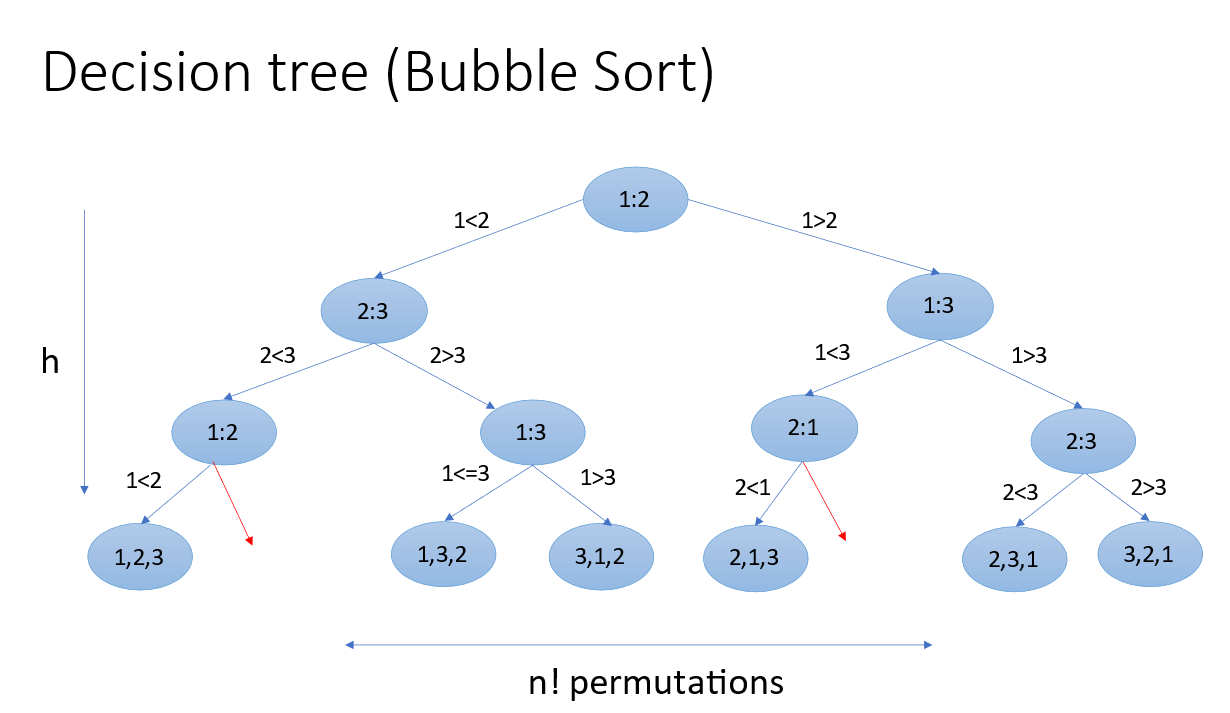
\includegraphics[scale=0.4]{wc02_image.png}    
\end{center}
Take $n=3$ and compare the efficiency of selection sort and insertion sort, in terms of the number of comparisons, with the help of a decision tree when the array is:
\begin{enumerate}
    \item Fully sorted
    \item Fully unsorted
\end{enumerate}

Please draw the decision tree for both algorithms and give your analysis in three to four lines.
\begin{solution}
\end{solution}
\end{questions}
\end{document}
